\section{IPython, le Python interactif}
\subsection{Les fonctionnalités}

\begin{frame}
  \frametitle{Fonctionnalités}
  \begin{itemize}
    \item Exécution de code dynamique
    \item Interaction avec le système
    \item Historique des commandes
    \item Journalisation
  \end{itemize}
\end{frame}

\subsection{Utile pour \ldots}
\begin{frame}[fragile]
  \frametitle{Utile pour \ldots}
    \begin{itemize}
      \item apprendre la syntaxe
    \end{itemize}
  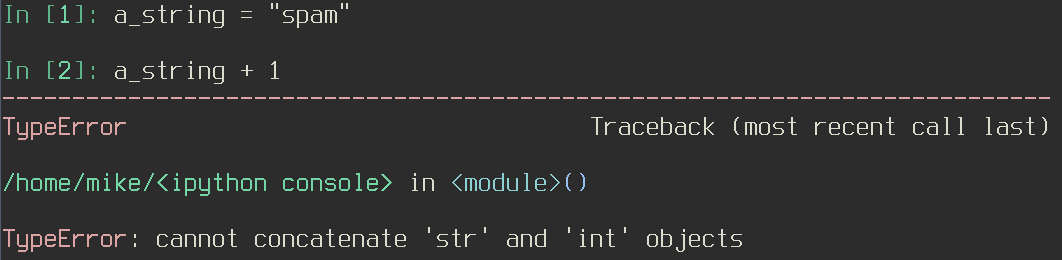
\includegraphics[scale=0.35]{apprendre.png}

\end{frame}

\begin{frame}
  \frametitle{Utile pour \ldots}
    \begin{itemize}
      \item prototyper une fonctionnalité
    \end{itemize}
    %note feth:
    % 1)
    %plutôt qu'un getter sur une var publique
    %je suggère une fonction qui fasse quelque chose, comme
    %def greet(self, name):
    %    return "%s greets %s." (self.name, name)
    % à votre avis ?
    %
    % 2) mentionner le ducktyping ? (à votre avis)
    % 2.1) Pour être callable il suffit d'implémenter 'def \_\_call\_\_(...)'
    % 2.2) pour être indexable : \_\_setitem\_\_(...), \_\_getitem\_\_(...)
    % Je ne sais pas trop comment insérer ça dans le cours, ça devrait venir plus tard dans le détail et c'est un peu hors sujet dans le prototypage..
  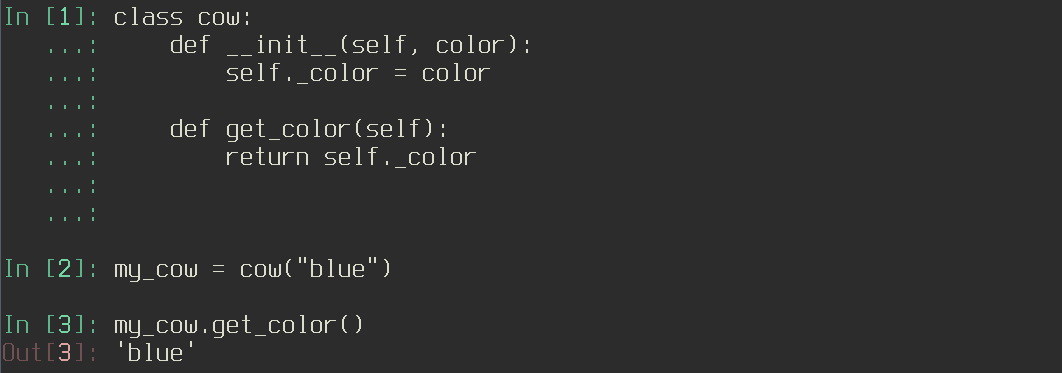
\includegraphics[scale=0.35]{prototype.png}
\end{frame}

\begin{frame}
  \frametitle{Utile pour \ldots}
    \begin{itemize}
      \item la découverte interactive d'une API
    \end{itemize}
  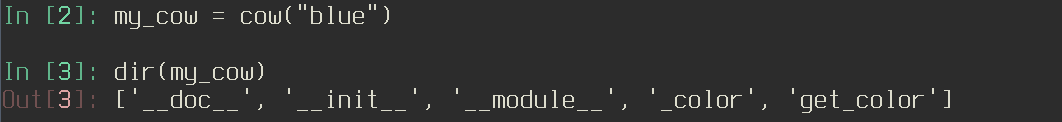
\includegraphics[scale=0.35]{api_discover.png}
\end{frame}

\begin{frame}
  \frametitle{Utile pour \ldots}
    \begin{itemize}
      \item embarquer un shell IPython dans ses programmes
    \end{itemize}
  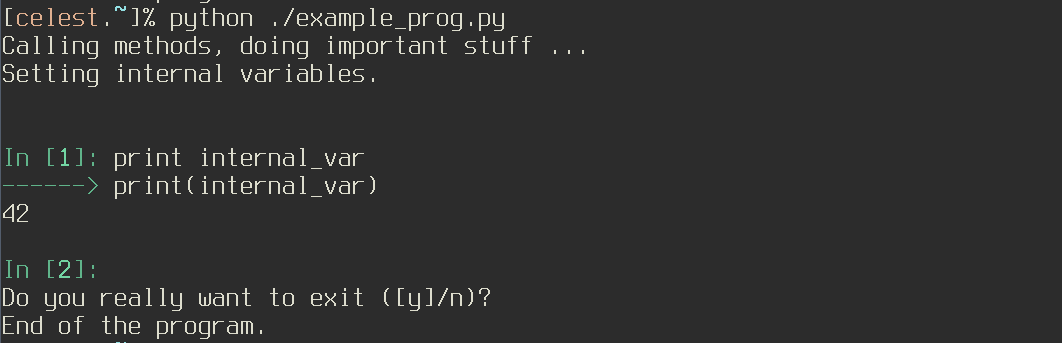
\includegraphics[scale=0.35]{embedded_ipython.png}
\end{frame}
